%----------------------------------------------------------------------------
\chapter{\projectlifecycle}
%----------------------------------------------------------------------------

A projektmenedzsment egyik alapvető elve, hogy minden projekt rendelkezik egy jól definiált életciklussal, 
amely több, egymásra épülő fázisra bontható. 
Ez az életciklus nemcsak logikai és időbeli folyamatot ír le, hanem szervezeti, irányítási és ellenőrzési szempontból is meghatározó, 
hiszen lehetővé teszi a projekt strukturált tervezését, a folyamatok nyomon követését, a kockázatok kezelését és a teljesítmény értékelését \cite{Szalay2018,Hajdu2014,Kaposi2019}. 

A hazai szakirodalom rendszerint öt alapvető fázist különít el \cite{Kovacs2016,Simon2015}:

\begin{enumerate}
    \item \textbf{Projektindítás (Initiation):} a projekt céljainak, indokoltságának, és a legfontosabb paraméterek meghatározása.
    \item \textbf{Tervezés (Planning):} részletes ütemezés, erőforrás-tervezés, kockázatelemzés és feladatdefiniálás.
    \item \textbf{Megvalósítás (Execution):} a projekt tényleges kivitelezése, fejlesztés és implementáció.
    \item \textbf{Ellenőrzés és irányítás (Monitoring \& Controlling):} az előrehaladás, a költségek, az idő és a minőség folyamatos követése.
    \item \textbf{Lezárás (Closure):} a projekt hivatalos befejezése, átadás, visszacsatolás és tapasztalatok dokumentálása.
\end{enumerate}

%----------------------------------------------------------------------------
\begin{figure}[H]
    \centering
    
\includegraphics[width=55mm, keepaspectratio]{figures/project_creative.png}
    \caption{Projekt kreatív vizualizáció}
    \label{fig:project_creative}
\end{figure}
%----------------------------------------------------------------------------

A fázisok egymásra épülnek, de gyakran átfedésben is zajlanak: például az ellenőrzési és irányítási tevékenység a megvalósítás teljes időtartama alatt folyamatosan jelen van. 
A modern, iteratív fejlesztési modellek — mint az Agile vagy Scrum — nem feltétlenül követik a klasszikus lineáris struktúrát, 
hanem sprint-alapú, ciklikus megközelítést alkalmaznak \cite{Hajdu2014,Kaposi2019}.

A klasszikus ötfázisú modell azonban stratégiai és vállalati projekteknél továbbra is nélkülözhetetlen, 
mivel átlátható keretet biztosít a projekt teljes életciklusára. 
A \textbf{TeDeRMS} fejlesztése során is ez a modell szolgált alapul, amelyet a projekt sajátosságaihoz — önálló fejlesztés, korlátozott erőforrások és vállalati integráció — igazítottam.

%----------------------------------------------------------------------------
\section{Projektindítás (Initiation)}
%----------------------------------------------------------------------------

A projektindítás szakasza a projekt életciklusának alapvető lépése, mivel meghatározza a projekt céljait, irányát és kereteit. 
A kezdeti fázis során végzett tevékenységek minősége közvetlen hatással van a projekt kockázatkezelésére, a mérföldkövek elérésére és a költséghatékonyságra. 
A projekt sikeressége nagymértékben függ a kezdeti igényfeltárás alapos elvégzésétől \cite{Hajdu2014,Szalay2018,Kovacs2016,Kaposi2019}.

\begin{itemize}
    \item \textbf{Igényfelmérés:} a vállalat bérléskezelési folyamatait részletesen feltérképeztem, azonosítva a problémás pontokat, és meghatározva a rendszer követelményeit \cite{Szalay2018}.
\end{itemize}

Az igényfelmérés célja a folyamatok és problémás területek feltárása, amely biztosítja a projekt következő szakaszainak sikeres végrehajtását. 
A részletes igényfeltárás segít a kockázatok korai azonosításában és a funkciók a valós vállalati igényekhez való illesztésében. 
Emellett fontos a szervezeti kontextus és az érintettek szempontjainak figyelembevétele, mivel ez növeli a projekt elfogadottságát és a végrehajtás hatékonyságát \cite{Kovacs2016,Kaposi2019}.

\begin{itemize}
    \item \textbf{Célok meghatározása:} világos, mérhető célokat tűztem ki, például az adminisztrációs idő csökkentését, az adatpontosság javítását és az automatizált riportok bevezetését.
\end{itemize}

A célok meghatározása biztosítja a projekt fókuszát és elősegíti az erőforrások optimális elosztását. 
A világos, mérhető célok lehetővé teszik a projekt mérföldköveinek nyomon követését és a teljesítmény objektív értékelését. 
A célok hierarchikus rendszere támogatja a stratégiai, taktikai és operatív döntések összehangolását, valamint a projektmenedzsment folyamatok átláthatóságát \cite{Hajdu2014,Szalay2018}.

\begin{itemize}
    \item \textbf{Erőforrás-tervezés előkészítése:} meghatároztam a projekt technológiai és időbeli erőforrásigényét. 
    Az önálló fejlesztés miatt kiemelten fontos volt a prioritások és a munkaidő hatékony beosztása.
\end{itemize}

Az erőforrás-tervezés előkészítése lehetővé teszi a rendelkezésre álló kapacitások optimális elosztását, 
a munkafolyamatok hatékony szervezését, valamint a prioritások meghatározását. 
A részletes erőforrás-tervezés segíti a rugalmasság biztosítását, a váratlan események kezelését, 
és elősegíti a mérföldkövek teljesítését a tervezett idő- és költségkereten belül \cite{Kovacs2016,Kaposi2019,Hajdu2014}.
A gondos projektindítás tehát stratégiai jelentőségű, mivel biztosítja a projekt későbbi fázisainak sikeres végrehajtását, 
miközben minimalizálja a félreértésekből és az erőforráspazarlásból eredő kockázatokat \cite{Szalay2018}.


%----------------------------------------------------------------------------
\section{Tervezés (Planning)}
%----------------------------------------------------------------------------

A tervezés szakasza kritikus jelentőségű a projekt sikerének biztosításában, mivel ekkor kerülnek meghatározásra az ütemezés, az erőforrások elosztása és a kockázatok kezelése. 
A részletes és előrelátó tervezés segít minimalizálni a váratlan problémák hatását, előre jelzi a potenciális kockázatokat, 
és lehetővé teszi a projekt teljesítményének nyomon követését \cite{Hajdu2014,Szalay2018,Kovacs2016,Kaposi2019}.

\begin{itemize}
    \item \textbf{Ütemterv készítése:} a projekt fő mérföldköveit és feladatait logikai és időbeli sorrendbe állítottam, így a fejlesztés előrehaladása követhetővé vált.
\end{itemize}

Az ütemterv elkészítése során a feladatok időbeli és logikai összefüggéseinek feltárása lehetővé teszi a projekt átláthatóságát és a folyamatok szisztematikus követését. 
A jól felépített ütemterv hozzájárul a mérföldkövek teljesítésének ellenőrzéséhez, 
és segít az erőforrások hatékony allokálásában \cite{Kovacs2016,Kaposi2019}. Emellett az ütemterv biztosítja a projekt 
előrehaladásának dokumentálását, amely elengedhetetlen a projektmenedzsment ellenőrzési folyamataihoz.

\begin{itemize}
    \item \textbf{Erőforrás-tervezés:} a napi és technológiai erőforrások meghatározása, a munkabeosztás optimalizálása biztosította az önálló fejlesztés gördülékenységét.
\end{itemize}

Az erőforrás-tervezés során a rendelkezésre álló humán és technológiai kapacitások felmérése és optimális elosztása kulcsfontosságú. 
A részletes erőforrás-tervezés lehetővé teszi a projekt rugalmasságát, 
elősegíti a prioritások meghatározását, és csökkenti a késedelmek kockázatát \cite{Hajdu2014,Szalay2018}. 
Különösen kiscsapatos vagy önálló fejlesztési környezetben a munkabeosztás és a rendelkezésre álló idő hatékony kezelése elengedhetetlen a projekt gördülékeny megvalósításához.

%----------------------------------------------------------------------------
\begin{figure}[H]
    \centering
    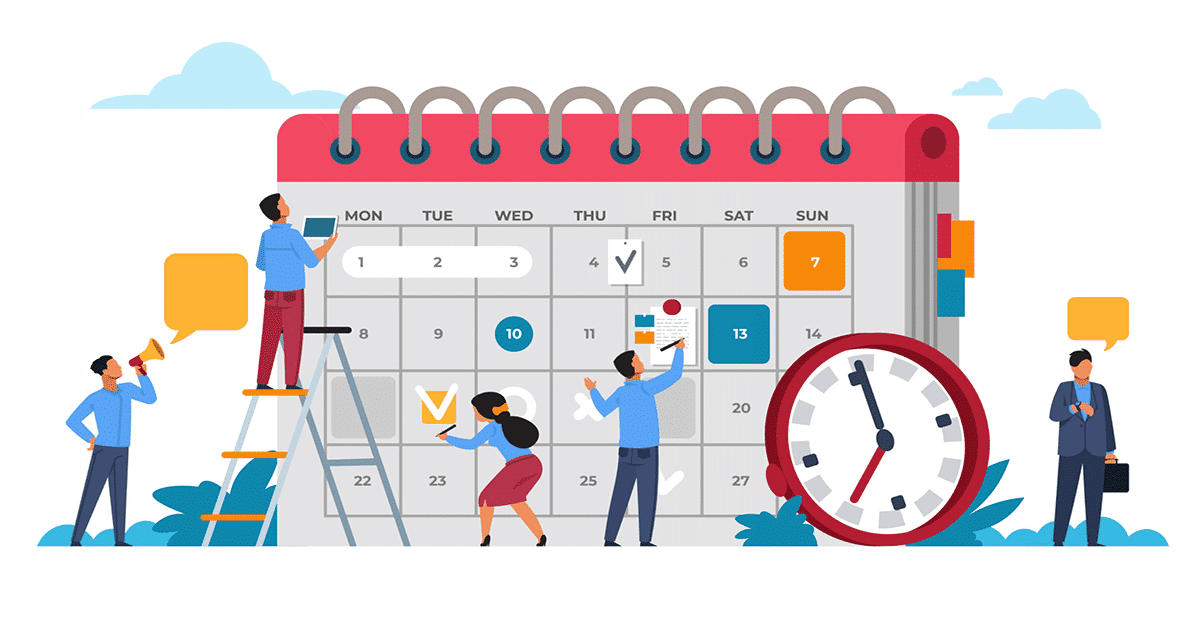
\includegraphics[width=70mm, keepaspectratio]{figures/plan.png}
    \caption{Naptári ütemterv vizualizáció}
    \label{fig:plan}
\end{figure}
%----------------------------------------------------------------------------

\begin{itemize}
    \item \textbf{Kockázatelemzés:} azonosítottam a fő kockázatokat (technikai hibák, adatvesztés, üzleti logika hibák), és kidolgoztam a megelőző és elhárító intézkedéseket.
\end{itemize}

A kockázatelemzés során feltárt potenciális problémák előrejelzése és kezelési tervének kidolgozása elengedhetetlen a projekt biztonságos és hatékony végrehajtásához. 
A kockázatmátrix alkalmazása lehetővé teszi a valószínűség és a hatás értékelését, és segíti a megelőző intézkedések priorizálását \cite{Kovacs2016,Kaposi2019}. 
Ez a megközelítés hozzájárul a projekt stabilitásához, és minimalizálja a váratlan események negatív következményeit.
A tervezési szakasz során alkalmazott módszerek, mint a feladatlista, az ütemezett mérföldkövek és a kockázatmátrix, 
valamint a folyamatos önellenőrzés és visszacsatolás, biztosítják a projekt strukturált és ellenőrizhető előrehaladását \cite{Hajdu2014,Szalay2018}.


%----------------------------------------------------------------------------
\section{Megvalósítás (Execution)}
%----------------------------------------------------------------------------

A megvalósítás szakasza a projekt tényleges kivitelezését foglalja magában, amely során a tervezett funkciók, 
folyamatok és erőforrások gyakorlati alkalmazásra kerülnek. Ebben a fázisban a projektmenedzsment 
és a technikai végrehajtás szoros összhangja kulcsfontosságú a kívánt eredmények eléréséhez \cite{Hajdu2014,Szalay2018,Kaposi2019}.

\begin{itemize}
    \item \textbf{Fejlesztési folyamatok:} moduláris architektúra kialakítása, backend és frontend párhuzamos fejlesztése, verziókövetés GitHub-on.
\end{itemize}

A moduláris architektúra lehetővé teszi a fejlesztési folyamatok párhuzamosítását, a hibák izolálását és a könnyebb karbantartást. 
A moduláris felépítés, valamint a verziókövető rendszerek alkalmazása elősegíti 
a projekt kontrollját, biztosítja a kód integritását és csökkenti a fejlesztési hibák számát \cite{Kovacs2016,Kaposi2019}. 
A backend és frontend párhuzamos fejlesztése hatékonyabb erőforrás-kezelést és gyorsabb fejlesztési ütemet tesz lehetővé.

\begin{itemize}
    \item \textbf{Tesztelés:} folyamatos unit és funkcionális tesztek, a rendszer stabilitásának és megbízhatóságának biztosítására.
\end{itemize}

A tesztelés kiemelt jelentőségű a megvalósítás során, mivel biztosítja a rendszer funkcionalitását, stabilitását 
és a hibamentes működést. A folyamatos tesztelés csökkenti a hibák későbbi 
előfordulásának kockázatát, és elősegíti a fejlesztés iteratív javítását, valamint 
a minőségbiztosítási folyamatok integrációját \cite{Szalay2018,Hajdu2014}. 
A unit tesztek elsősorban az egyes modulok helyes működését ellenőrzik, míg a funkcionális tesztek a teljes rendszer üzleti logikáját vizsgálják.

\begin{itemize}
    \item \textbf{Dokumentáció:} részletes kód- és rendszer-dokumentáció, amely elősegíti a későbbi karbantartást és bővítést.
\end{itemize}

A dokumentáció a projekt hosszú távú fenntarthatóságának alapfeltétele. A kód és 
rendszer részletes dokumentálása nemcsak a karbantartást és bővítést könnyíti meg, hanem elősegíti a tudás megőrzését, 
a fejlesztői csapat tagjai közötti kommunikációt, és támogatja az esetleges auditok vagy rendszerellenőrzések lebonyolítását \cite{Kovacs2016,Kaposi2019,Szalay2018}.
A megvalósítás szakasz tehát biztosítja, hogy a rendszer minden funkciója a tervek szerint valósuljon meg, és a vállalat 
igényeit teljes mértékben kielégítse, miközben a projektmenedzsment eszközök és a dokumentáció révén a folyamat átlátható és ellenőrizhető marad \cite{Hajdu2014}.


%----------------------------------------------------------------------------
\section{Ellenőrzés és irányítás (Monitoring és Controlling)}
%----------------------------------------------------------------------------

Az ellenőrzés és irányítás fázisa a projekt sikerének egyik legfontosabb garanciája, mivel biztosítja, 
hogy a tervezett célok és mérföldkövek teljesüljenek, az erőforrások optimálisan legyenek felhasználva, 
és a projekt kockázatai időben kezelhetők legyenek \cite{Hajdu2014,Szalay2018,Kovacs2016,Kaposi2019}. 
A monitoring és controlling nemcsak a problémák azonosítását 
szolgálja, hanem lehetővé teszi a proaktív beavatkozást és a projekt folyamatos optimalizálását.

\begin{itemize}
    \item \textbf{Haladás nyomon követése:} mérföldkövek teljesülésének ellenőrzése, eltérések azonosítása és korrekciója.
\end{itemize}

A haladás nyomon követése során a mérföldkövek teljesítését folyamatosan ellenőrizni kell, hogy a projekt 
a tervezett ütemterv szerint haladjon. A rendszeres ellenőrzés lehetővé teszi 
a korai eltérések azonosítását, a késedelmek és a túlzott erőforrás-felhasználás megelőzését, valamint 
támogatja a szükséges korrekciók gyors végrehajtását \cite{Kovacs2016,Kaposi2019}. 
A mérföldkövek objektív értékelése javítja a projekt átláthatóságát és a vezetői döntések megalapozottságát.

\begin{itemize}
    \item \textbf{Kockázatok kezelése:} a kockázatmátrix folyamatos frissítése, a problémák gyors és hatékony megoldása.
\end{itemize}

A kockázatok folyamatos kezelése lehetővé teszi, hogy a potenciális problémák hatása minimalizálható legyen. 
A kockázatmátrix rendszeres frissítése segít az új kockázatok azonosításában, 
a valószínűség és hatás értékelésében, valamint a megelőző intézkedések és vészforgatókönyvek kidolgozásában \cite{Hajdu2014,Szalay2018}. 
A proaktív kockázatkezelés csökkenti a projekt idő- és költségkeretének túllépésének esélyét, és növeli a projekt sikerességét.

%----------------------------------------------------------------------------
\begin{figure}[H]
    \centering
    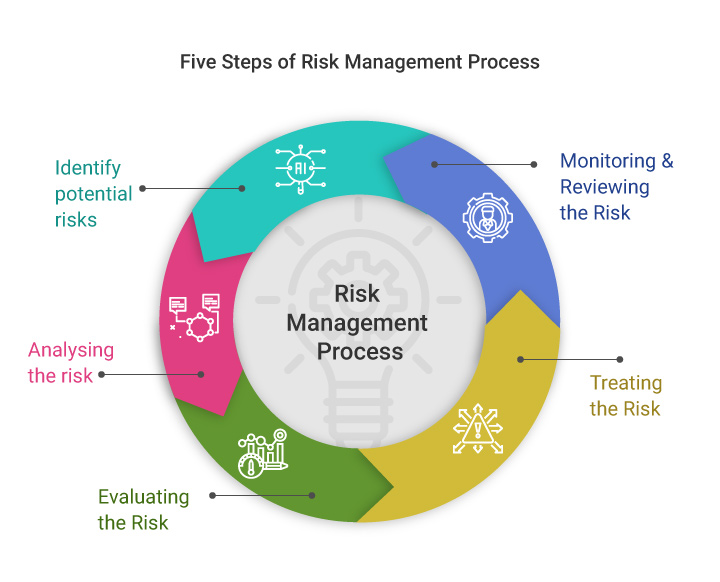
\includegraphics[width=70mm, keepaspectratio]{figures/risk.jpg}
    \caption{Kockázatkezelés példa}
    \label{fig:risk}
\end{figure}
%----------------------------------------------------------------------------

\begin{itemize}
    \item \textbf{Minőségellenőrzés:} a rendszer funkcionalitásának és stabilitásának folyamatos ellenőrzése a hibák minimalizálása érdekében.
\end{itemize}

A minőségellenőrzés célja, hogy a projekt kimenete megfeleljen a tervezett specifikációknak, és a hibák a lehető 
legkorábban kerüljenek azonosításra. A folyamatos minőségellenőrzés biztosítja a rendszer 
stabilitását és megbízhatóságát, támogatja az iteratív javításokat, és hozzájárul a projekt végső sikeréhez \cite{Kovacs2016,Kaposi2019,Szalay2018}.
Az ellenőrzés és irányítás tehát kulcsfontosságú a projekt kereteinek betartásában, a mérföldkövek teljesítésében és a 
kívánt minőség biztosításában, miközben lehetőséget nyújt a folyamatos optimalizálásra és a kockázatok proaktív kezelésére.


%----------------------------------------------------------------------------
\section{Projekt lezárás (Closure)}
%----------------------------------------------------------------------------

A projekt lezárása a projektmenedzsment egyik kritikus fázisa, mivel ekkor valósul meg a fejlesztett 
rendszer végső átadása, a tapasztalatok összegzése és a hosszú távú fenntarthatóság biztosítása. 
A lezárás során történő alapos értékelés és dokumentáció 
kulcsfontosságú a projekt teljesítményének, hatékonyságának és minőségének fenntartásához \cite{Hajdu2014,Szalay2018,Kovacs2016,Kaposi2019}.

\begin{itemize}
    \item \textbf{Rendszer átadása:} a \textbf{TeDeRMS} teljes körű telepítése a vállalat környezetében.
\end{itemize}

A rendszer átadása során a telepítésnek zökkenőmentesen kell biztosítania a teljes funkcionalitást a 
vállalati környezetben. Az átadás minősége és pontossága közvetlen hatással 
van a felhasználói elfogadásra, a napi operatív folyamatokra és a projekt hosszú távú sikerére \cite{Szalay2018,Kovacs2016}. 
A hibamentes átadás elősegíti a vállalati folyamatok zavartalan működését, és csökkenti a támogatási igényeket.

\begin{itemize}
    \item \textbf{Dokumentáció:} részletes felhasználói és adminisztrátori kézikönyvek készítése.
\end{itemize}

A dokumentáció a hosszú távú fenntarthatóság záloga, mivel biztosítja, hogy a rendszer működését és 
konfigurációját később bárki könnyen megérthesse és kezelhesse. 
A dokumentáció nemcsak a felhasználók számára nyújt útmutatót, hanem a 
karbantartást és a jövőbeli fejlesztéseket is támogatja, valamint alapot ad a rendszer auditálásához \cite{Hajdu2014,Kaposi2019}.

\begin{itemize}
    \item \textbf{Oktatás:} a kulcsfelhasználók képzése a rendszer hatékony használatára.
\end{itemize}

A képzés biztosítja, hogy a rendszer a vállalatnál maximális hatékonysággal legyen alkalmazható. 
A felhasználói oktatás közvetlenül hozzájárul a rendszer elfogadásához, 
a hibák csökkentéséhez és a napi működés zavartalanságához \cite{Szalay2018,Kovacs2016}. 
Az oktatás során szerzett ismeretek elősegítik a rendszer önálló kezelését és a belső támogatási igény minimalizálását.

\begin{itemize}
    \item \textbf{Tanulságok összegzése:} a projekt során szerzett tapasztalatok dokumentálása és javaslatok a jövőbeli fejlesztésekhez.
\end{itemize}

A projekt lezárása során a tanulságok összegzése lehetővé teszi a szervezeti tudás megőrzését és a folyamatok fejlesztését. 
A tapasztalatok dokumentálása segíti a jövőbeli projektek tervezését, a hibák elkerülését 
és a hatékonyabb projektmenedzsment kialakítását \cite{Hajdu2014,Szalay2018,Kaposi2019}. 
Ez a tudás hosszú távon növeli a vállalati projektek sikerességét és stabilitását.

A lezárási fázis tehát biztosítja, hogy a rendszer hosszú távon stabilan és hatékonyan működjön, 
miközben a projektmenedzsment tapasztalatai a későbbiekben is hasznosíthatók.

%----------------------------------------------------------------------------
\begin{figure}[H]
    \centering
    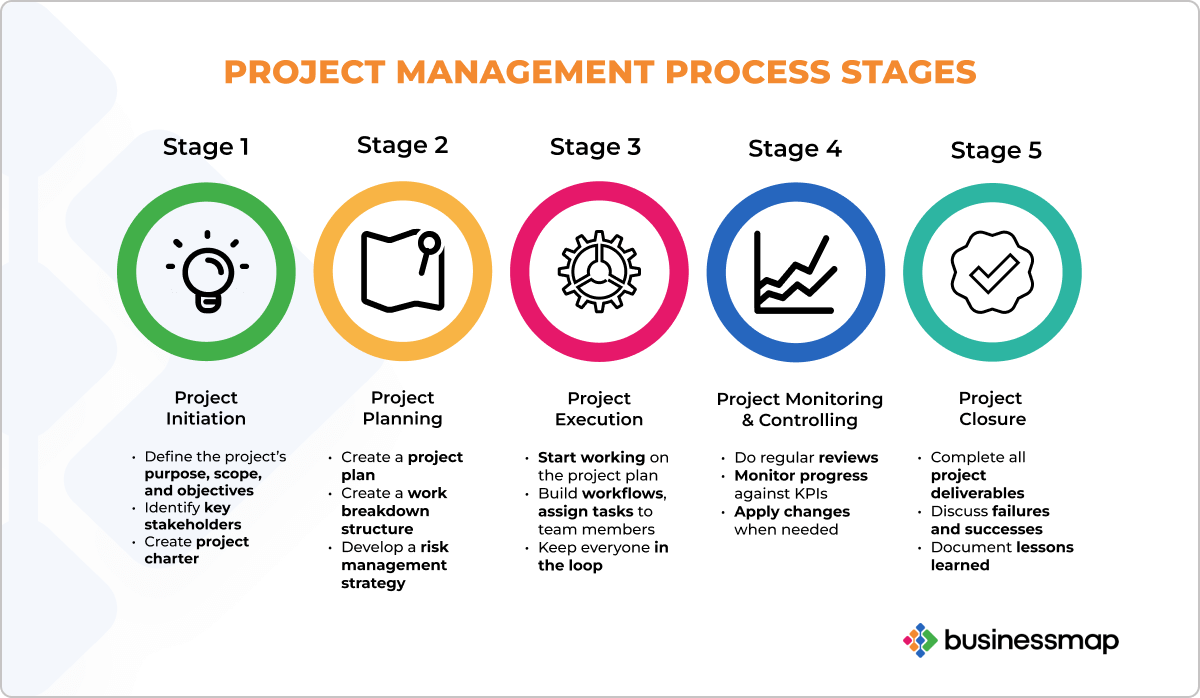
\includegraphics[width=130mm, keepaspectratio]{figures/project_management_process_stages.png}
    \caption{Projektmenedzsment folyamatok fázisai}
    \label{fig:project_management_process_stages}
\end{figure}
%----------------------------------------------------------------------------
